\documentclass{report}

\usepackage[english]{babel}
\usepackage[T1]{fontenc}
\usepackage[utf8]{inputenc}

\usepackage[pdfborder={0 0 0}]{hyperref}
\usepackage[dvipsnames]{xcolor}
\usepackage{graphicx}
\usepackage{array}
\usepackage{tabulary}
\usepackage[top=1.5cm, bottom=1.5cm, left=1.5cm, right=1.5cm]{geometry}
\usepackage{tikz}
\usepackage{menukeys}
\usepackage{multicol}
\usepackage{animate}
\usepackage{pdflscape}
\usepackage{listings}
\lstset{basicstyle=\ttfamily\color{darkgray},
		numbers=left,
		frame=single,
		breaklines=true,
		stringstyle=\color{PineGreen},
		commentstyle=\color{Tan},
		extendedchars=true,
		keywordstyle=\bfseries\color{RedOrange}}

\newcolumntype{M}{>{\centering\arraybackslash}m{\dimexpr.25\linewidth-2\tabcolsep}}

\title{Lorann-Ex}
\author{Baptiste Saclier\and Maire Chiaverini\and Clément Chabrier\and Maxime Zupka}
\date{Mercredi 23 Juin 2016}

\begin{document}

\maketitle

\tableofcontents
\clearpage

\chapter{Planning}

At the beginning of the project we had to organize all the project to give differents tasks to the members of the team.

\section{Team}

The team is composed of four persons each have a specific task in the project.

\begin{description}
\item[Baptiste Saclier] \emph{Project leader} : In charge of the organisation of the project and the controller of the software
\item[Marie Chiaverini] In charge of the model of the game, loading systems and data storage
\item[Clément Chabrier] In charge of the view of the project, UML redactor and documentation master
\item[Maxime Zupka] In charge of the design of the level, the documentation and the administration of the database.
\end{description}

\section{Planning diagram}


\begin{landscape}
\subsection{Estimated planning}
\vspace*{\fill}

\begin{center}
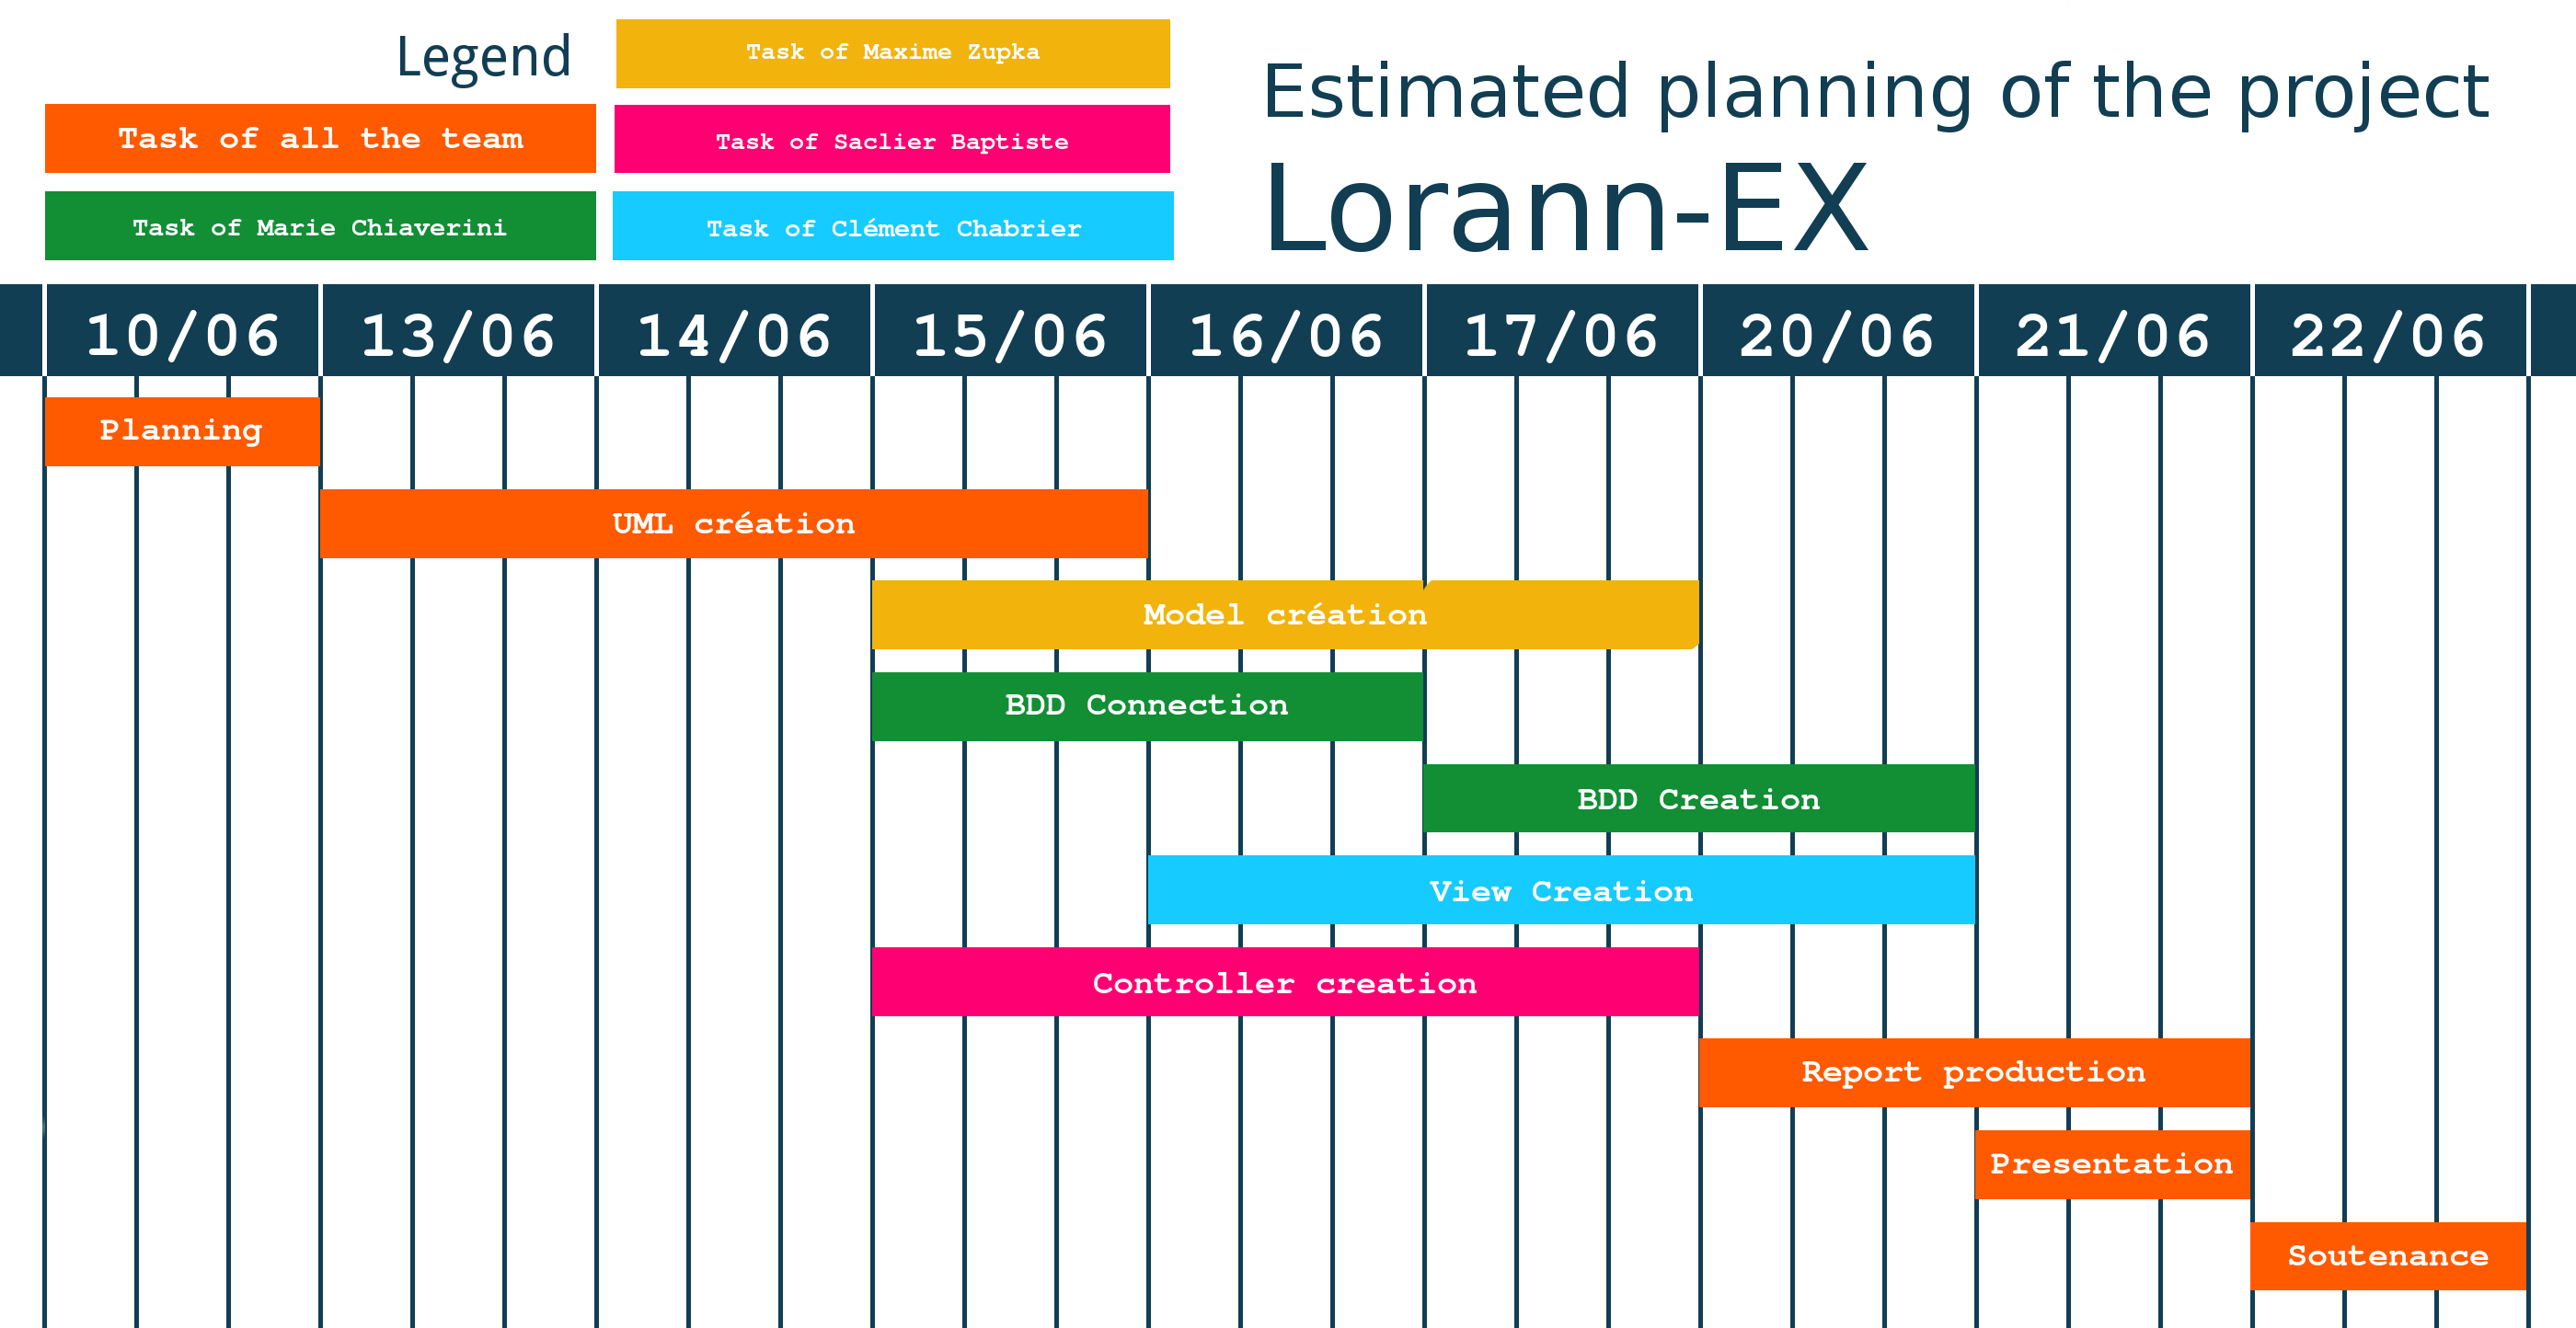
\includegraphics{resources/Planning-previsionnel.png}
\end{center}

\vspace*{\fill}

\end{landscape}

\begin{landscape}
\subsection{Efficient planning}
\vspace*{\fill}

\begin{center}
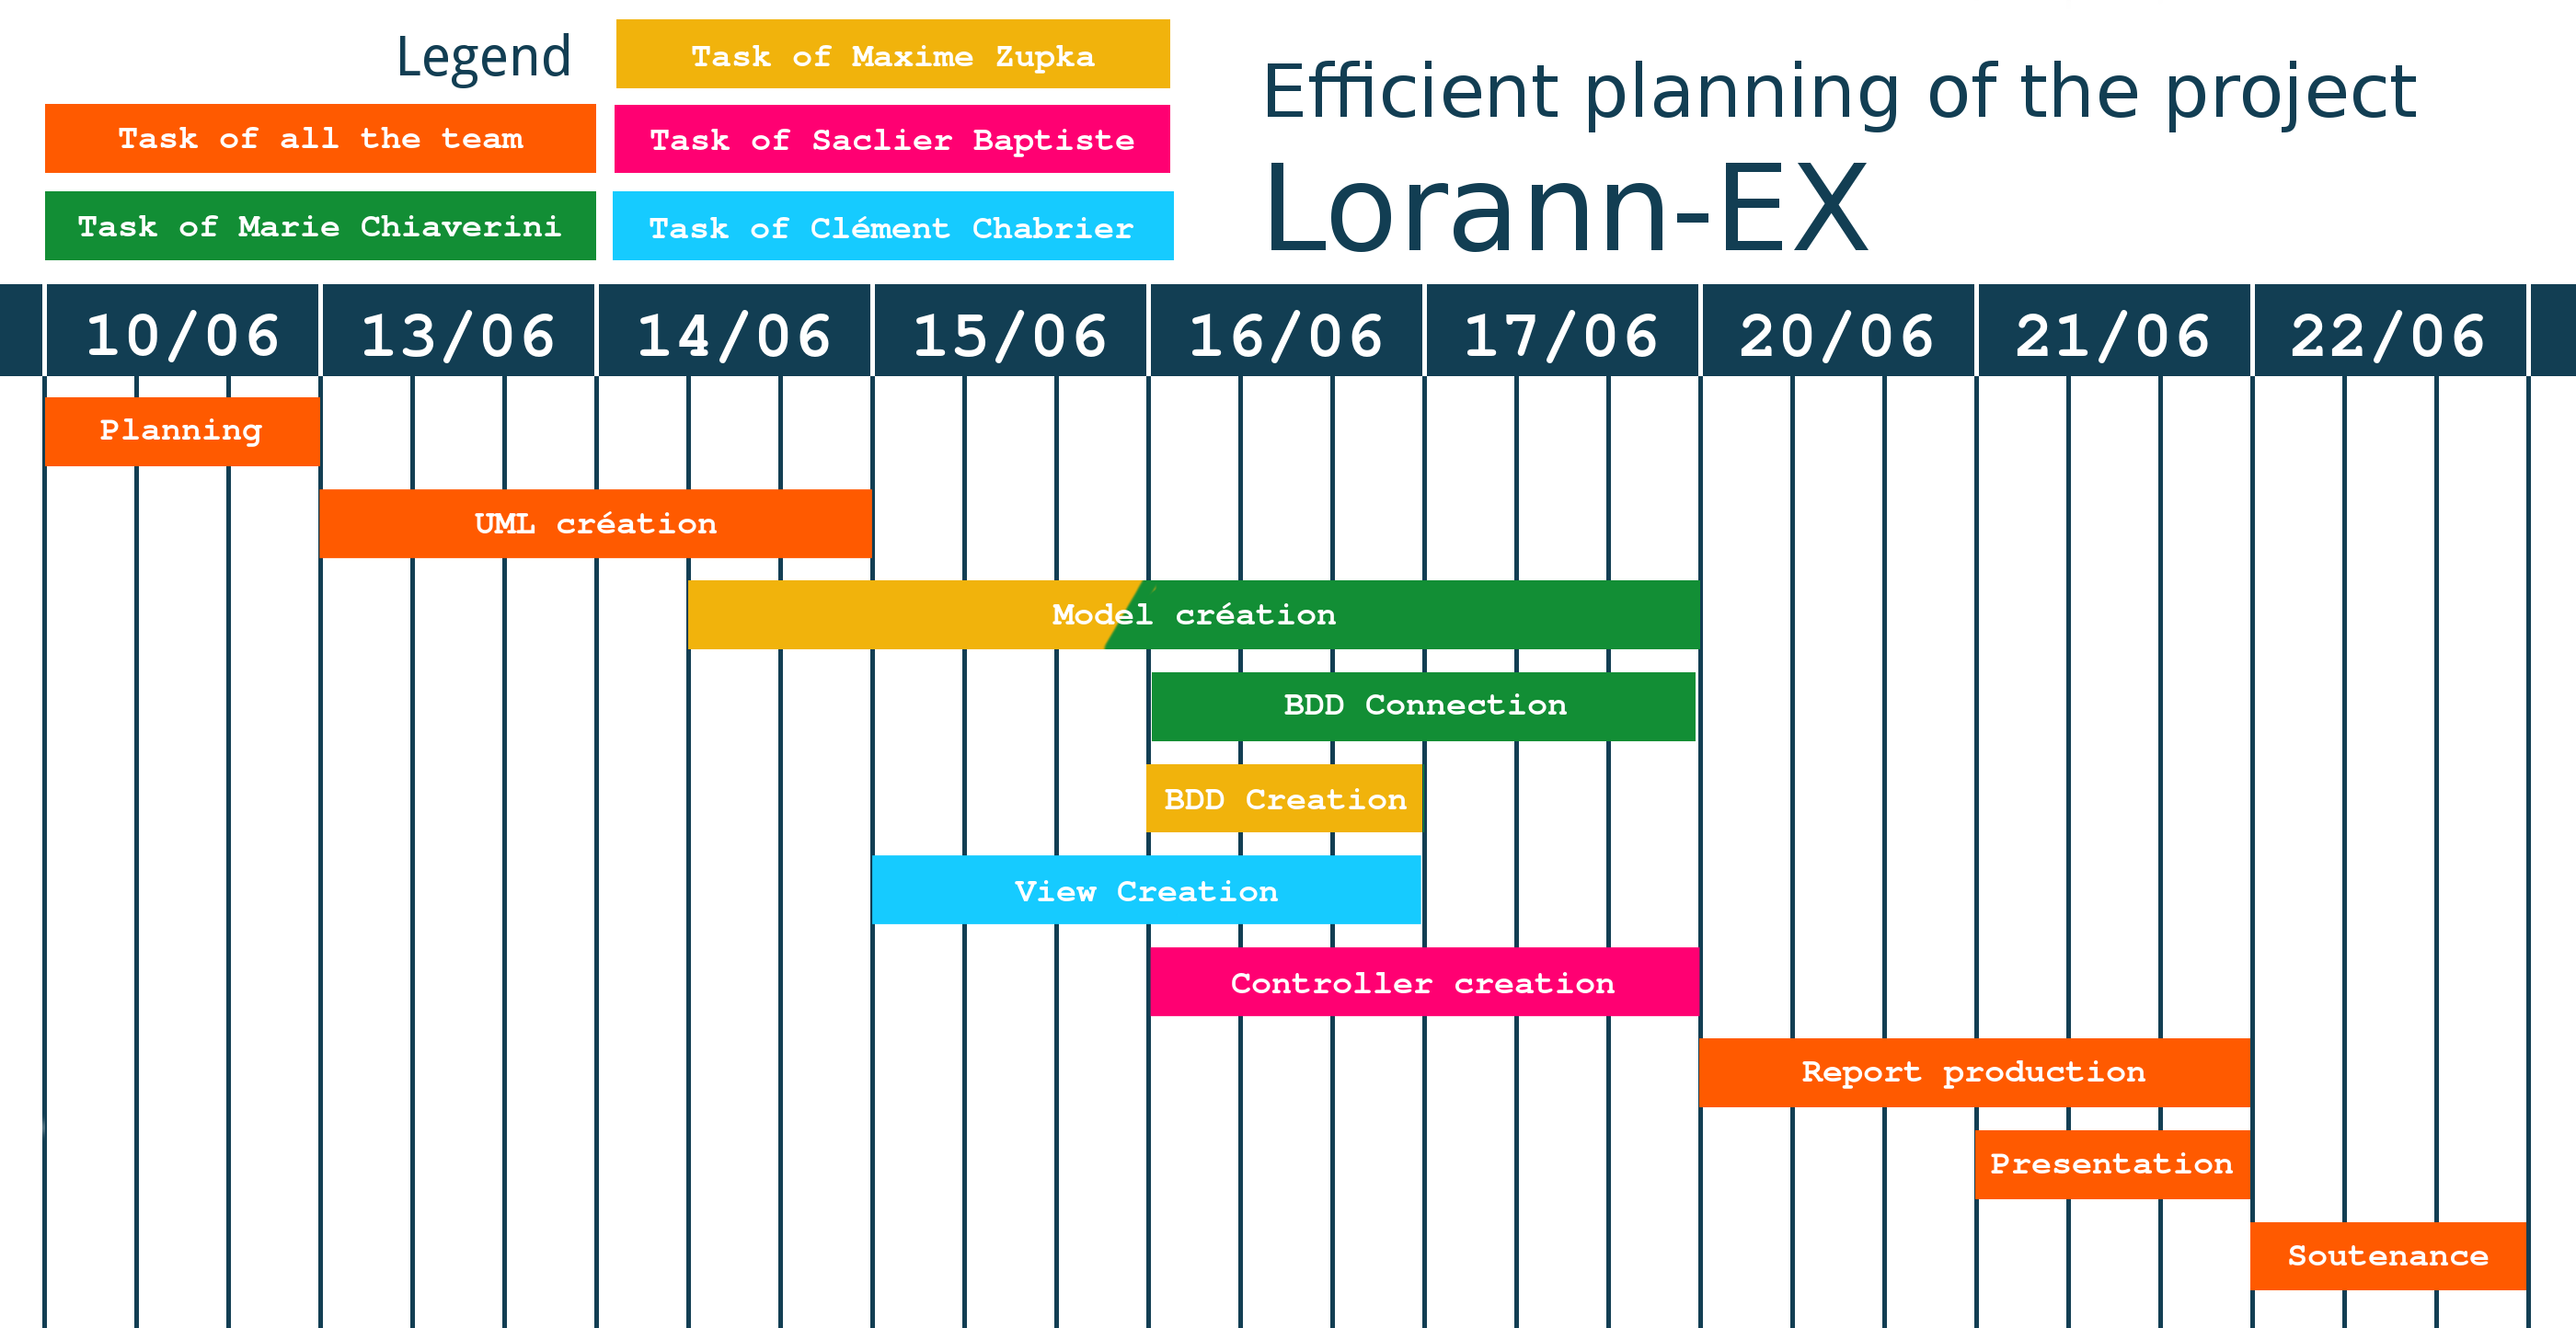
\includegraphics{resources/Planning-effectif.png}
\end{center}

\vspace*{\fill}s
\end{landscape}

\chapter{Game manual}

Welcome to the world of Lorann. In this dungeon you will discover a whole universe of danger in the maze of Nova-Ann. You have to finish all the levels to win the game.

Good luck Lorann.

\section{Installation}

The installation of the game is pretty easy. Just download the executable \emph{JAR} from \emph{github.com} at the address \texttt{\href{https://github.com/EpicKiwi/Lorann-Ex/releases/download/0.0.2/Lorann-Ex-0.0.2-SNAPSHOT.jar}{goo.gl/Mf4zIH}}. And play. The database is distant and fully configurated.

\section{Level}

\begin{center}
\textsf{The first level of the game}\par
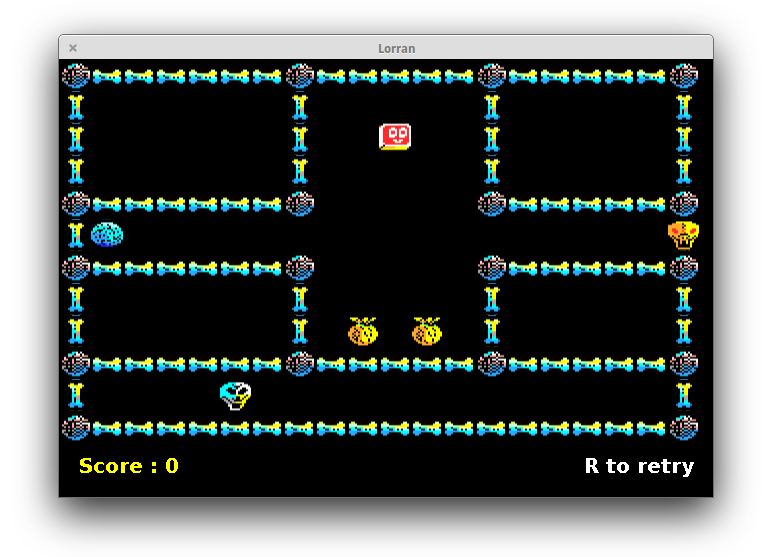
\includegraphics[scale=0.5]{resources/lvlorann.png}
\end{center}

A level contains many elements and each of them have a specific behavior. Next, you will find the components of this level and a short description of them.

\begin{center}
\begin{tabulary}{0.9\linewidth}{|c|c|L|}
\hline
Name & Sprite & Description \\
\hline
\hline
Lorann & 
\includegraphics[scale=0.7]{resources/sprites/lorann_b.png} & The hero of the game. You can control him to finish the level, kill monsters and earn points. \\
\hline
Wall & 
\includegraphics[scale=0.7]{resources/sprites/bone.png}
\includegraphics[scale=0.7]{resources/sprites/vertical_bone.png}
\includegraphics[scale=0.7]{resources/sprites/horizontal_bone.png} & The limits of the level. You and the monsters cannot pass trought this elements. \\
\hline
Purse & 
\includegraphics[scale=0.7]{resources/sprites/purse.png} & A 100 points bonus when lorann come from this item. \\
\hline
Magic Bubble & 
\includegraphics[scale=0.7]{resources/sprites/crystal_ball.png} & The key of the level. You need to get it to open the door and finish the level. \\
\hline
Door & 
\includegraphics[scale=0.7]{resources/sprites/gate_closed.png}
\includegraphics[scale=0.7]{resources/sprites/gate_open.png} & On the left, the door of the level closed. It will kill you if you step on it. On the right, the door opened. Yous can finish the level if you step on it. \\
\hline
Monster & 
\includegraphics[scale=0.7]{resources/sprites/monster_1.png}
\includegraphics[scale=0.7]{resources/sprites/monster_2.png}
\includegraphics[scale=0.7]{resources/sprites/monster_3.png}
\includegraphics[scale=0.7]{resources/sprites/monster_4.png} & The monster is a deadly element. You cannot step on it but you can shoot it by launching a spell. There are 4 types of monster specified in the section \ref{monsters}\\
\hline
\end{tabulary}
\end{center}

\paragraph{Goal} The goal of the level is to go out by the opened door. Opened by the Magic bubble you took just before.

\paragraph{Points} There are many possibilities to get points. First by taking money purses. By finishing the level, by taking the Magic bubble or by shooting monsters.

\section{Monsters}
\label{monsters}

There are four types of monsters. Each type have his own sprite and his own comportment. But they can all be killed by the spell of lorann and all killes lorann when he meet one of them.

\paragraph{Straight monster}
\hspace{\fill}
\includegraphics{resources/sprites/monster_1.png}

This type of monster just go in a direction UP, DOWN, LEFT or RIGHT and bounce on walls. By killing it you will earn 150 points.

\paragraph{Diagonal monster}
\hspace{\fill}
\includegraphics{resources/sprites/monster_2.png}

This type of monster go in a diagonal direction and bouce on the wall. If you kill it you will earn 225 points.

\paragraph{Random monster}
\hspace{\fill}
\includegraphics{resources/sprites/monster_3.png}

This type of monster go in a random direction at any time. This random monster take a new direction on each tick. If you kill it you will earn 285 points

\paragraph{Following monster}
\hspace{\fill}
\includegraphics{resources/sprites/monster_4.png}

This type of monster is the most dangerous. It will be follow Lorann in a straight line without avoid walls. If you kill it you will earn 315 points.

\section{Controls}

You have to control the position of lorann to go at the end of the level. To control him just use the arrow keys.

\begin{center}
\begin{tabular}{ccc}
& \keys{\arrowkeyup} & \\[4mm]
\keys{\arrowkeyleft} & \keys{\arrowkeydown} & \keys{\arrowkeyright} \\
\end{tabular}
\end{center}

\clearpage

You can allso use the standards french or american FPS keys like.

\begin{center}
\begin{multicols}{2}
\begin{tabular}{rrcll}
&& $\uparrow$ && \\[2mm]
&& \keys{Z} && \\[4mm]
$\leftarrow$ &\keys{Q} & \keys{S} & \keys{D}& $\rightarrow$ \\[2mm]
&& $\downarrow$ &&\\
\end{tabular}

\begin{tabular}{rrcll}
&& $\uparrow$ && \\[2mm]
&& \keys{W} && \\[4mm]
$\leftarrow$ &\keys{Q} & \keys{S} & \keys{D}& $\rightarrow$ \\[2mm]
&& $\downarrow$ &&\\
\end{tabular}
\end{multicols}
\end{center}

\section{Spell}

\begin{center}

\includegraphics{resources/sprites/fireball_1.png}
\includegraphics{resources/sprites/fireball_2.png}
\includegraphics{resources/sprites/fireball_3.png}
\includegraphics{resources/sprites/fireball_4.png}
\includegraphics{resources/sprites/fireball_5.png}
\end{center}

Lorann can cast a multicolor spell on the level to kill monsters by using the \keys{\Space space\Space} key. It will be lauch in front of lorann and will bounce on the walls.

If the spell hits Lorann he will be able to cast an other one. If it hits a monster, he will die and the spell continue his path.

\section{Retry}

If Lorann die you can restart the level from the beginning by hitting the key \keys{R}. Il will cost you 350 points and the level will be reloaded.

\chapter{Software's system}

\section{MVC}

The MVC (model-view-controller), is a data pattern used in JAVA to build efficiently softwares. It has the property of separate the program in three categories.

\subsection{Model}

The model part represents the software’s core, it shall treat the data and tell to the view what it should show to the user. 

In our case the model has multiple functions:

\begin{itemize}
\item To get data from the database
	\begin{itemize}
	\item DBProperties class
	\item DBConnection class
	\item Model class
	\end{itemize}
\item To build the level to play, set the elements to their location and define their properties
	\begin{itemize}
	\item Element class and all its derivatives
	\item Location class
	\item Level class
	\item Dimention class
	\item Direction enumeration
	\end{itemize}
\item To select what sprite will appear on screen
	\begin{itemize}
	\item Sprite
	\item AnimatedSprite
	\end{itemize}
\end{itemize}

to see a graphic view of the model unit please report to the next page.

\begin{landscape}

\vspace*{\fill}

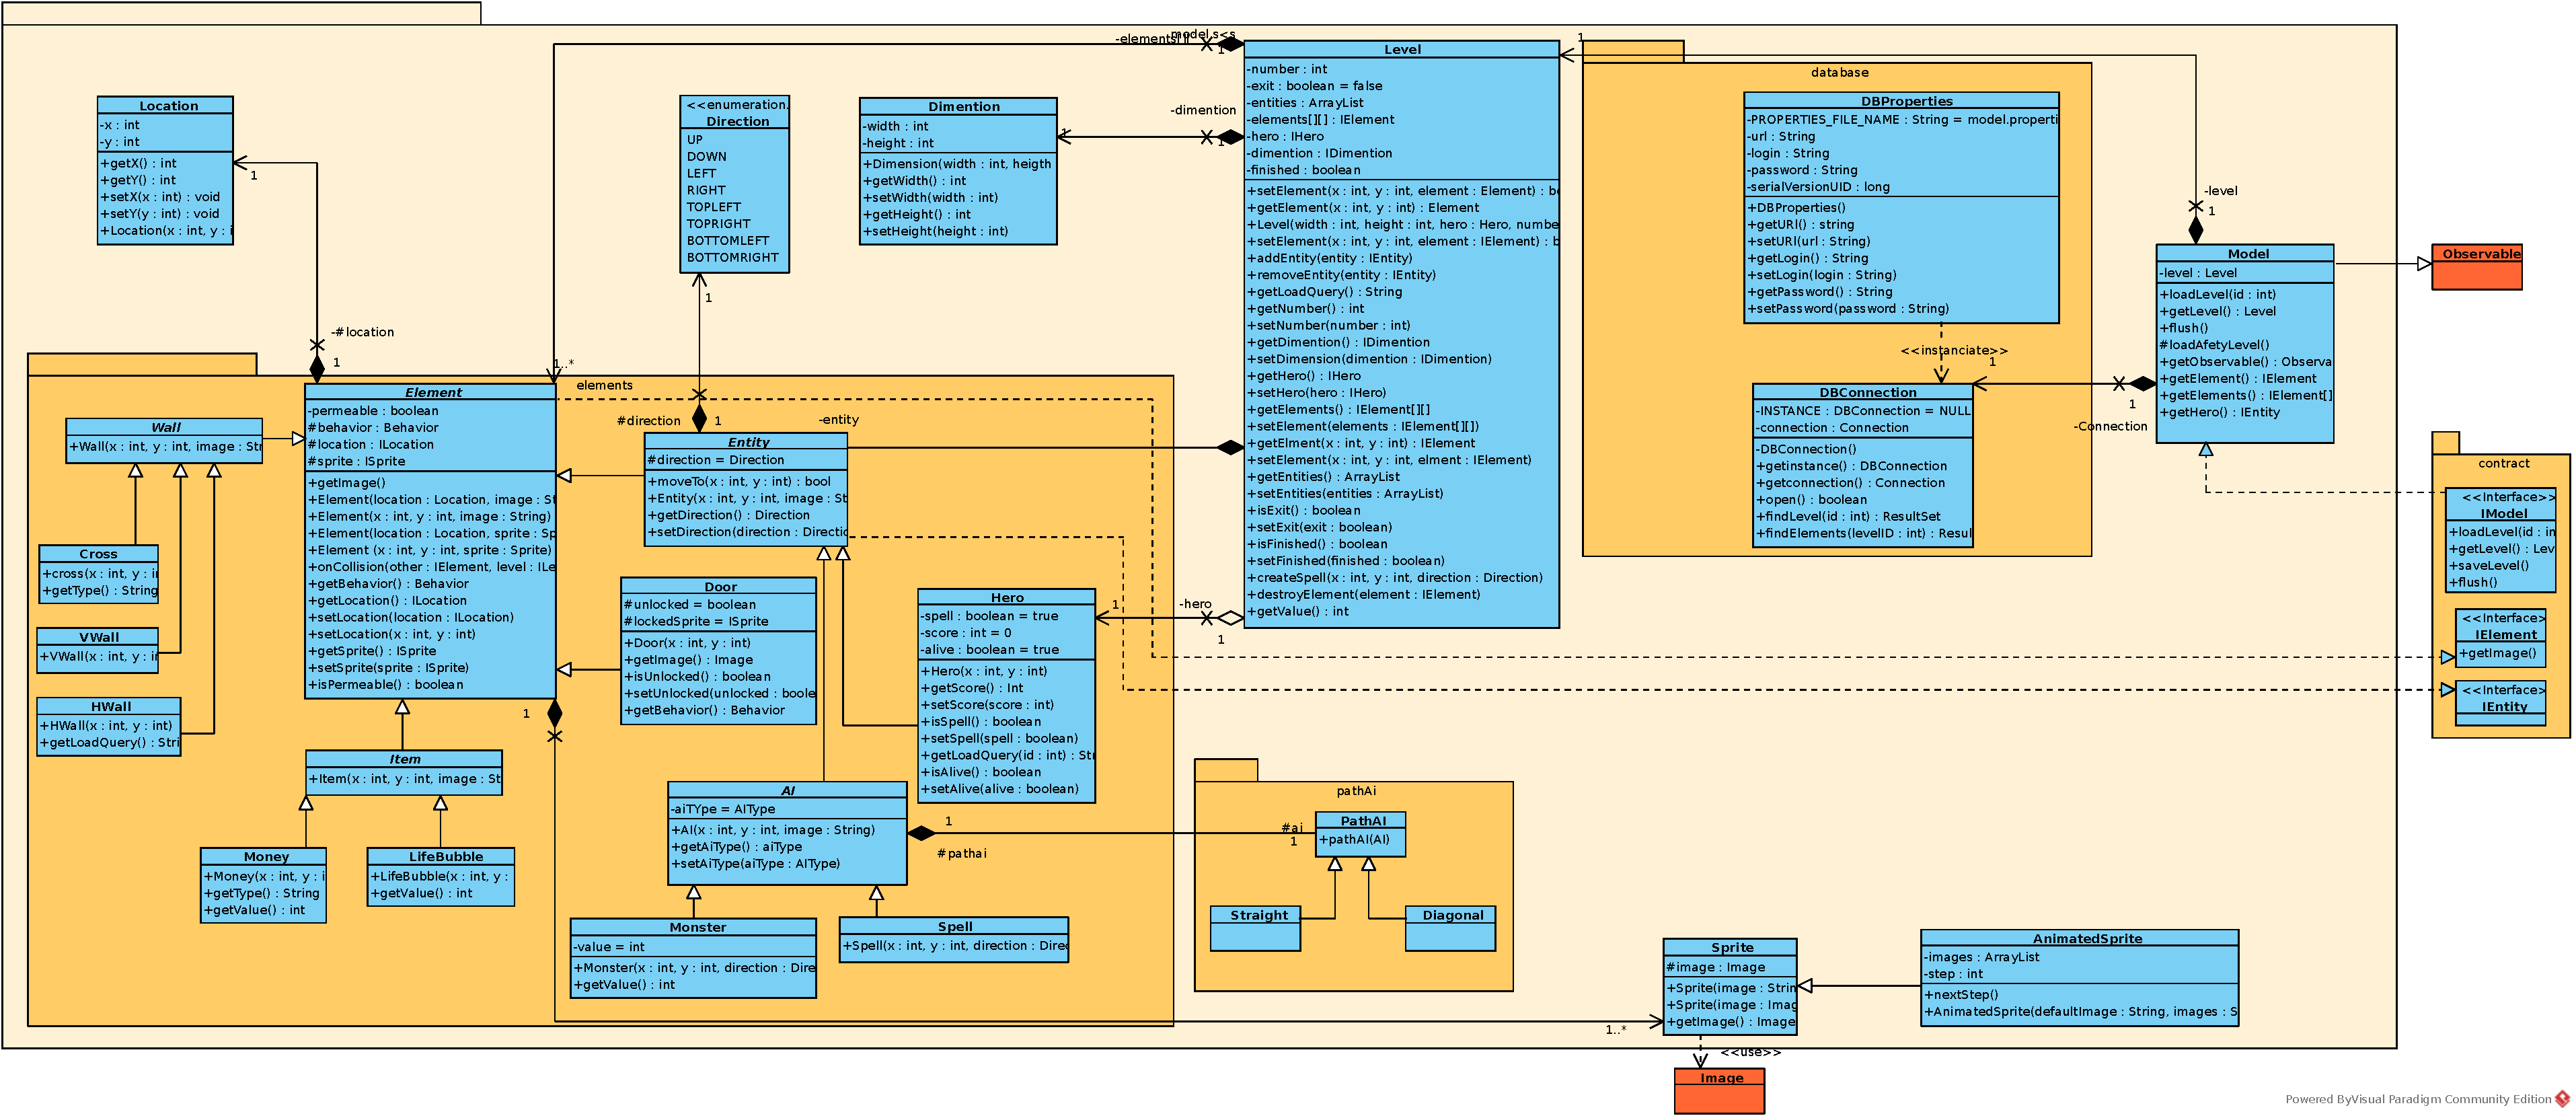
\includegraphics[scale=0.39]{resources/SVG/model.pdf}

\vspace*{\fill}

\end{landscape}

\subsection{View}

The view is the visual interface trough which one the user shall “see” the program.

It has to show the results of the calculations from the model unit and to “listen” every action from the user that may cause a change in the program (mouse click, key pressed etc…) 

In our game the view part:
\begin{itemize}
\item Open a frame to see the game
	\begin{itemize}
	\item GameFrame class
	\end{itemize}
\item Display graphic elements on the screen
	\begin{itemize}
	\item GamePanel class
	\end{itemize}
\item Update what the user see, based on the model’s information
	\begin{itemize}
	\item View class
	\end{itemize}
\item Keyes listener
	\begin{itemize}
	\item GameFrame class
	\end{itemize}
\end{itemize}

\paragraph{About the model and the view}

In order to inform the view unit about the model changments, we have to set up a pattern observer.
We create an observer interface that will notice the view every possible changes and will make it react, so the information on screen update in real time.

\bigskip

to see a graphic view of the view unit please report to the next page.

\begin{landscape}

\vspace*{\fill}

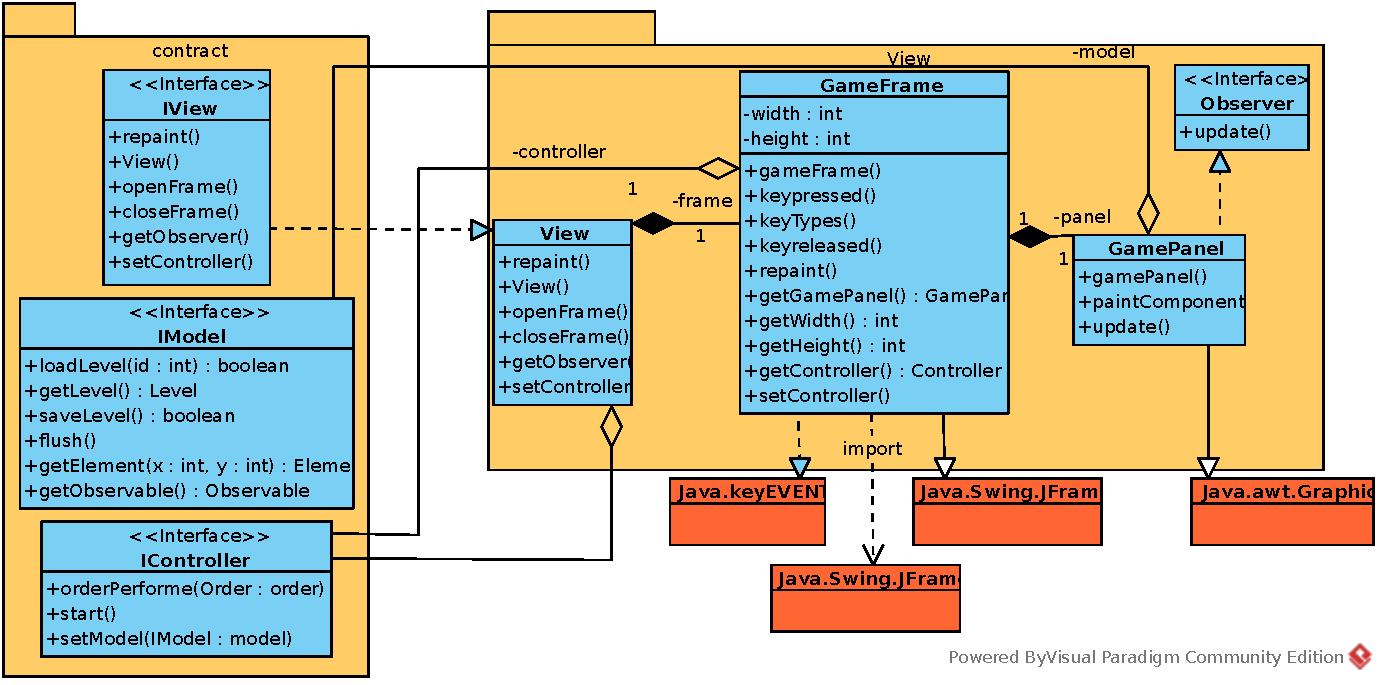
\includegraphics[scale=1.1]{resources/SVG/view.pdf}

\vspace*{\fill}

\end{landscape}

\subsection{Controller}

This part of the program is in charge of the event management. It has to synchronize every action in the software, in order update the view or the model correctly. 

It receives events from the view unit and treat the information in order to trigger the appropriate reaction from the model part.

In our program the controller has to:

\begin{itemize}
\item Start the game
	\begin{itemize}
	\item Controller class
	\end{itemize}
\item Synchronize the software’s actions
	\begin{itemize}
	\item Clock class
	\end{itemize}
\item Manage the behavior of every element that will appear on screen
	\begin{itemize}
	\item HeroManager class
	\item MoveManager class
	\item CollisionManager class
	\item AIManager class
	\end{itemize}
\item Inform the model of every order to perform and changes to apply
	\begin{itemize}
	\item Controller class
	\end{itemize}
\end{itemize}

to see a graphic view of the Controller unit please report to the next page.

\begin{landscape}

\vspace*{\fill}

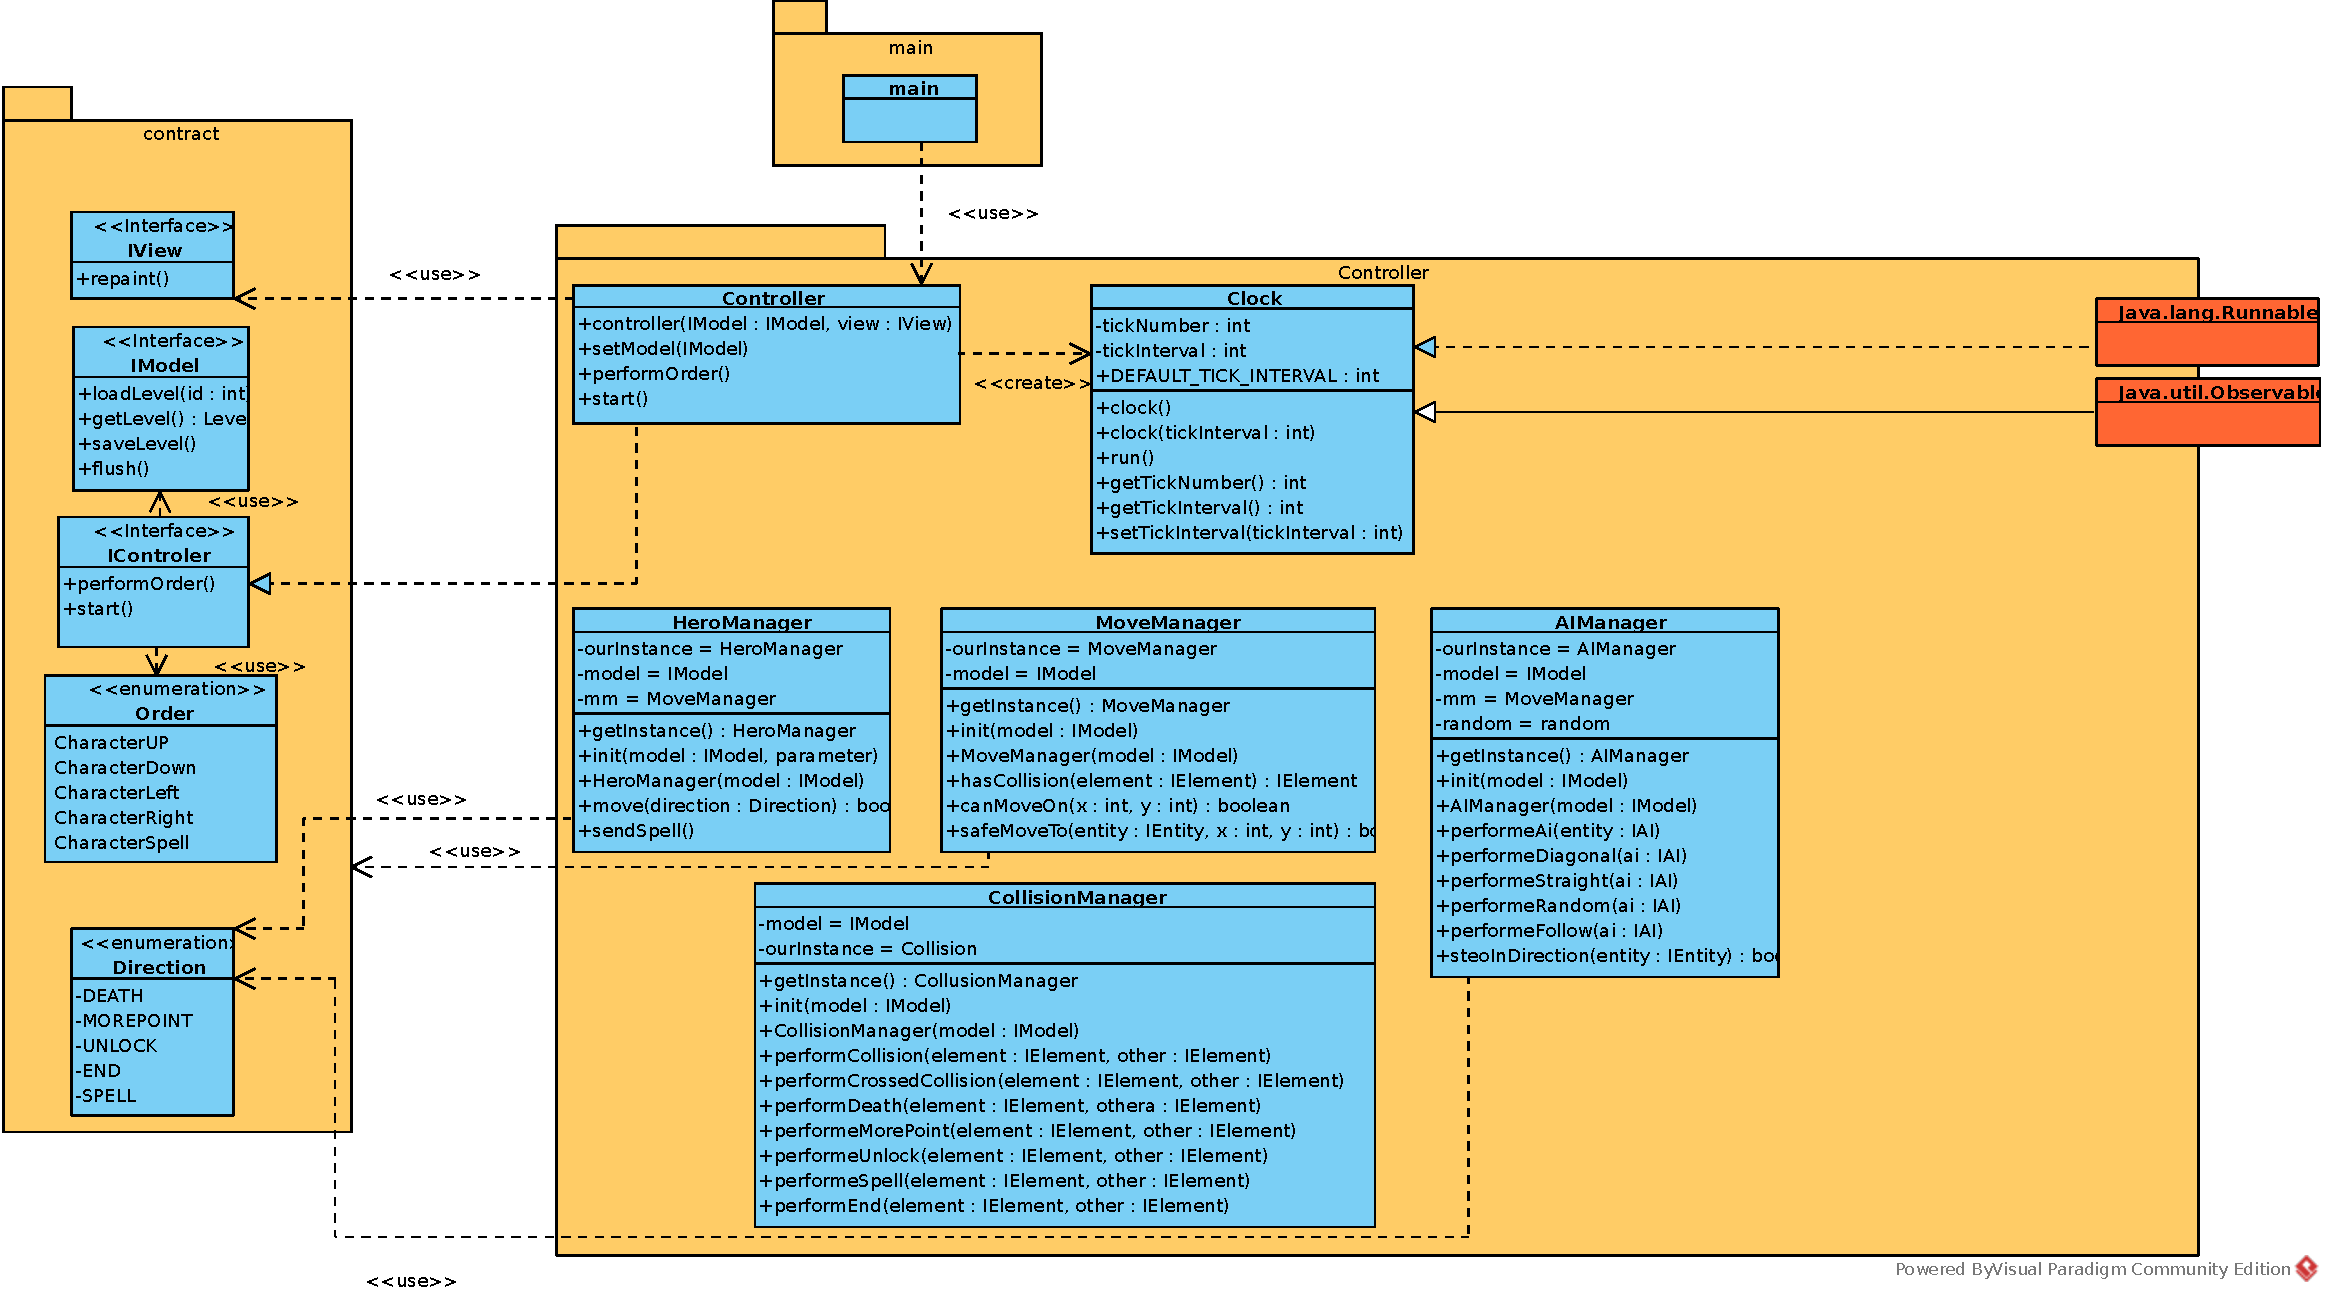
\includegraphics[scale=0.65]{resources/SVG/controler.pdf}

\vspace*{\fill}

\end{landscape}

\subsection{Contract}

A classic MVC pattern has a default, it creates a large number of couple between the three parts, that may cause program dysfunction and it decrease the code’s reusability.

In order to face those problems, wet set a fourth unit in our program, the contract. 

In this last part we create many interfaces within which contain operation from every class that has to be use in another part of the program than its native unit.

For example, the view needs information from the model, so it will use its interface, IModel.

to see a graphic view of the Contract unit please report to the next page.

\begin{landscape}

\vspace*{\fill}

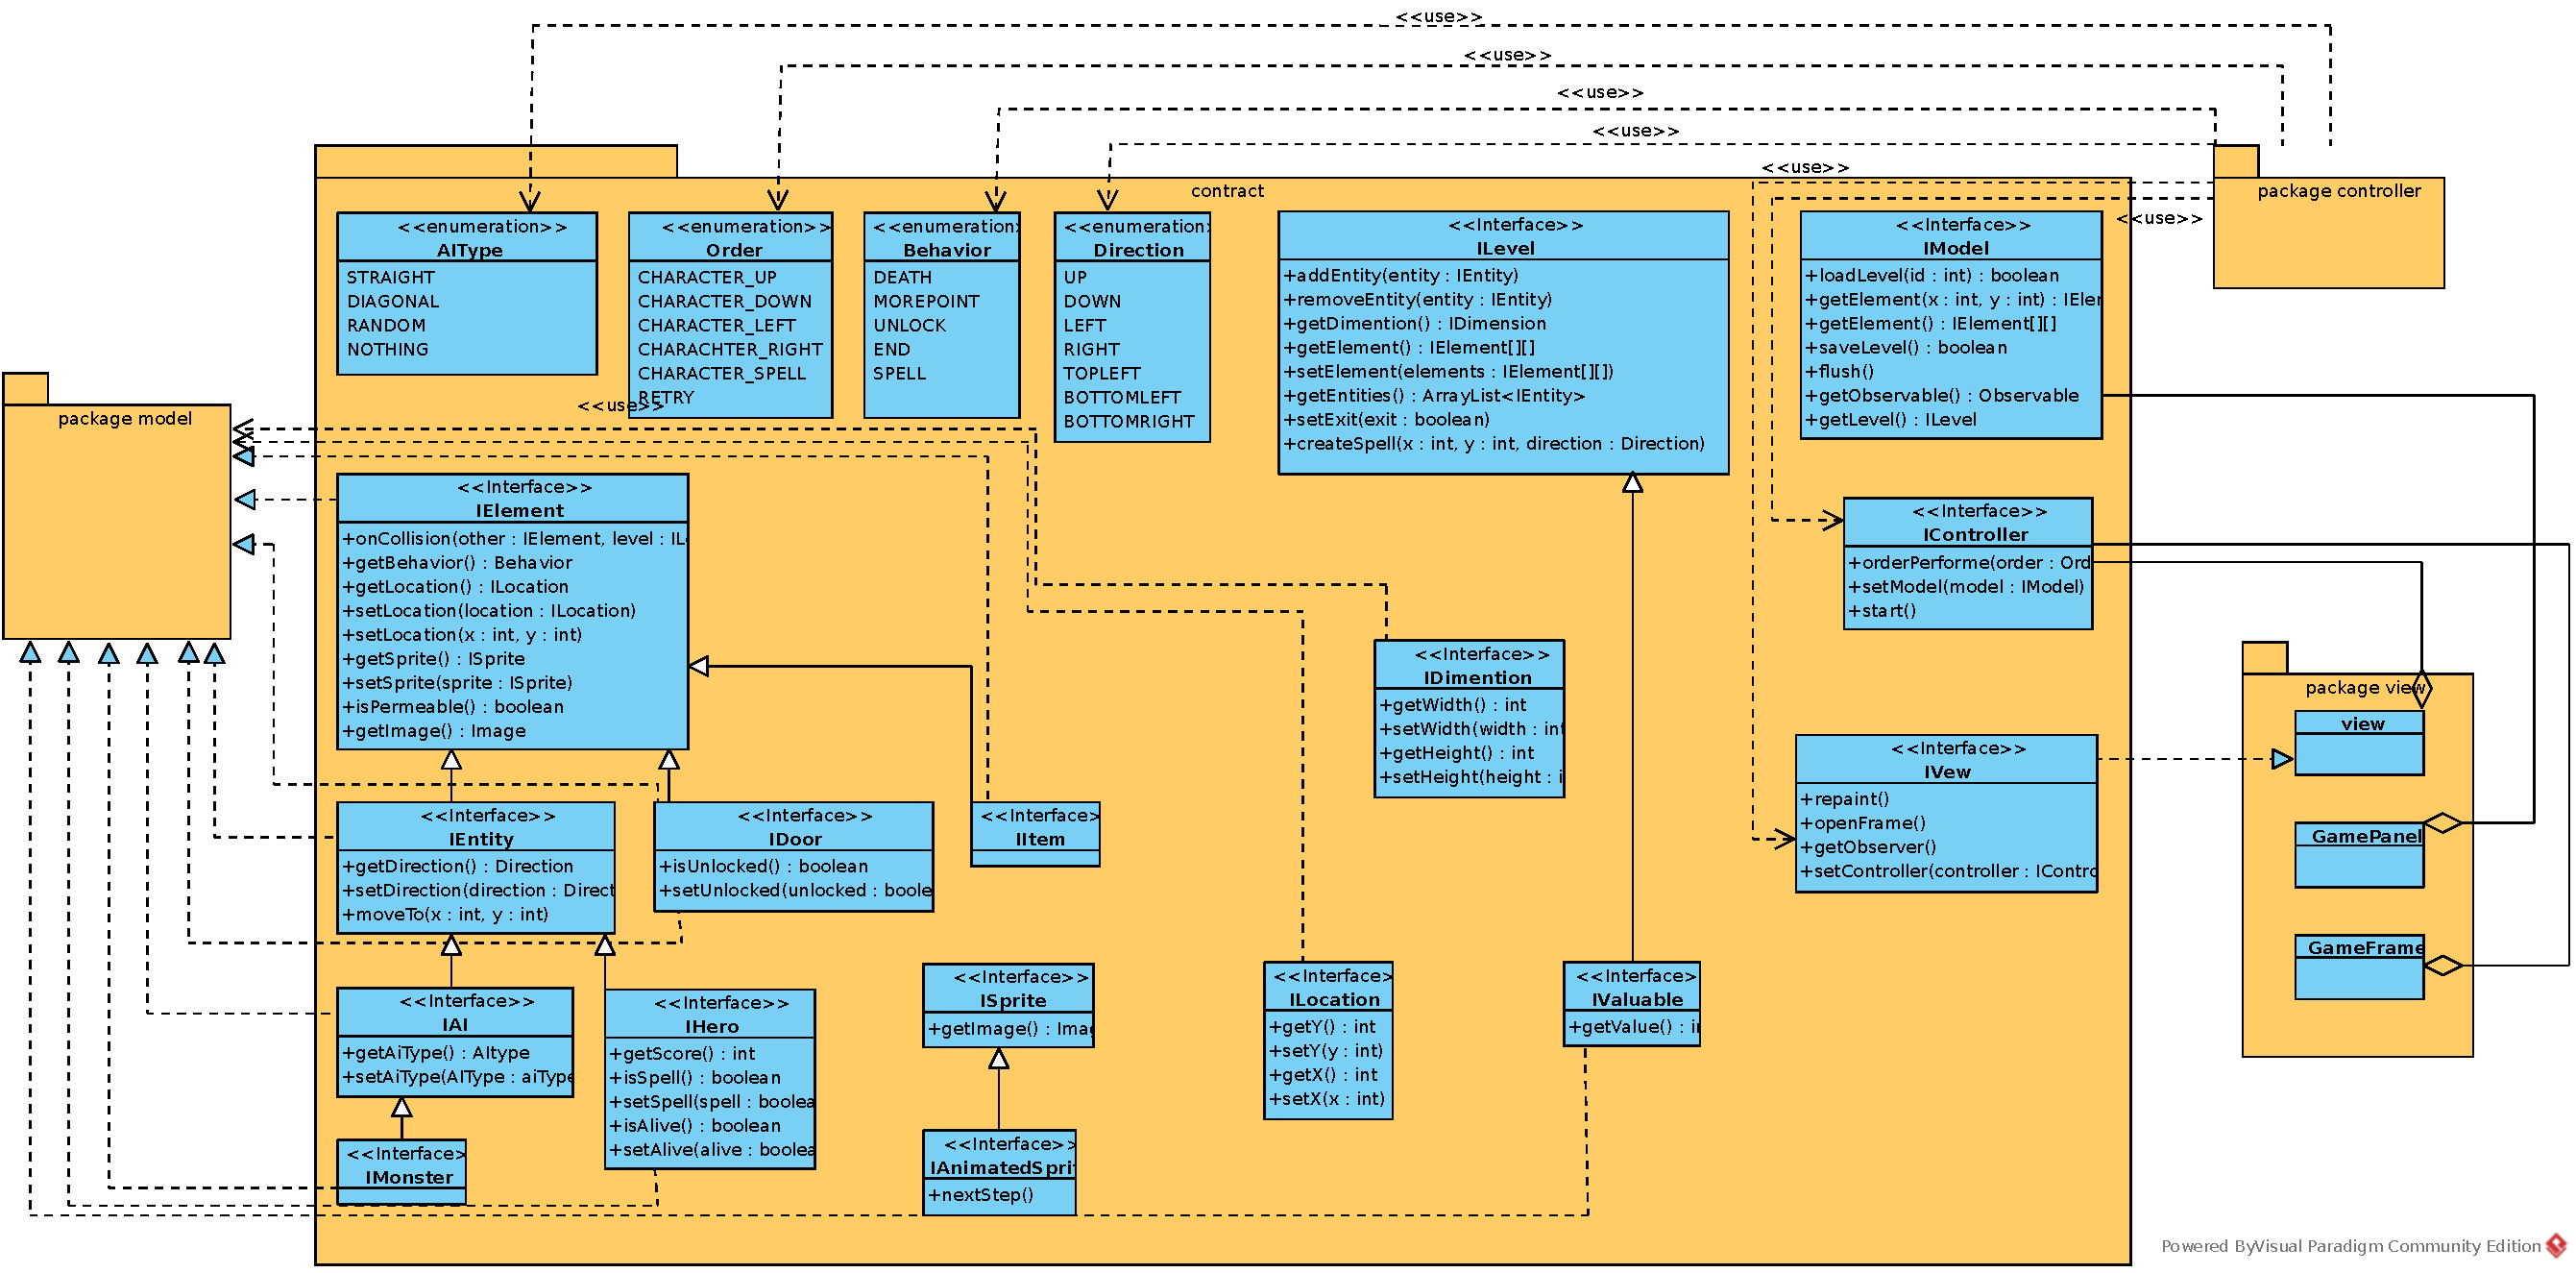
\includegraphics[scale=0.56]{resources/SVG/contract.pdf}

\vspace*{\fill}

\end{landscape}

\subsection{Packages}

\begin{center}
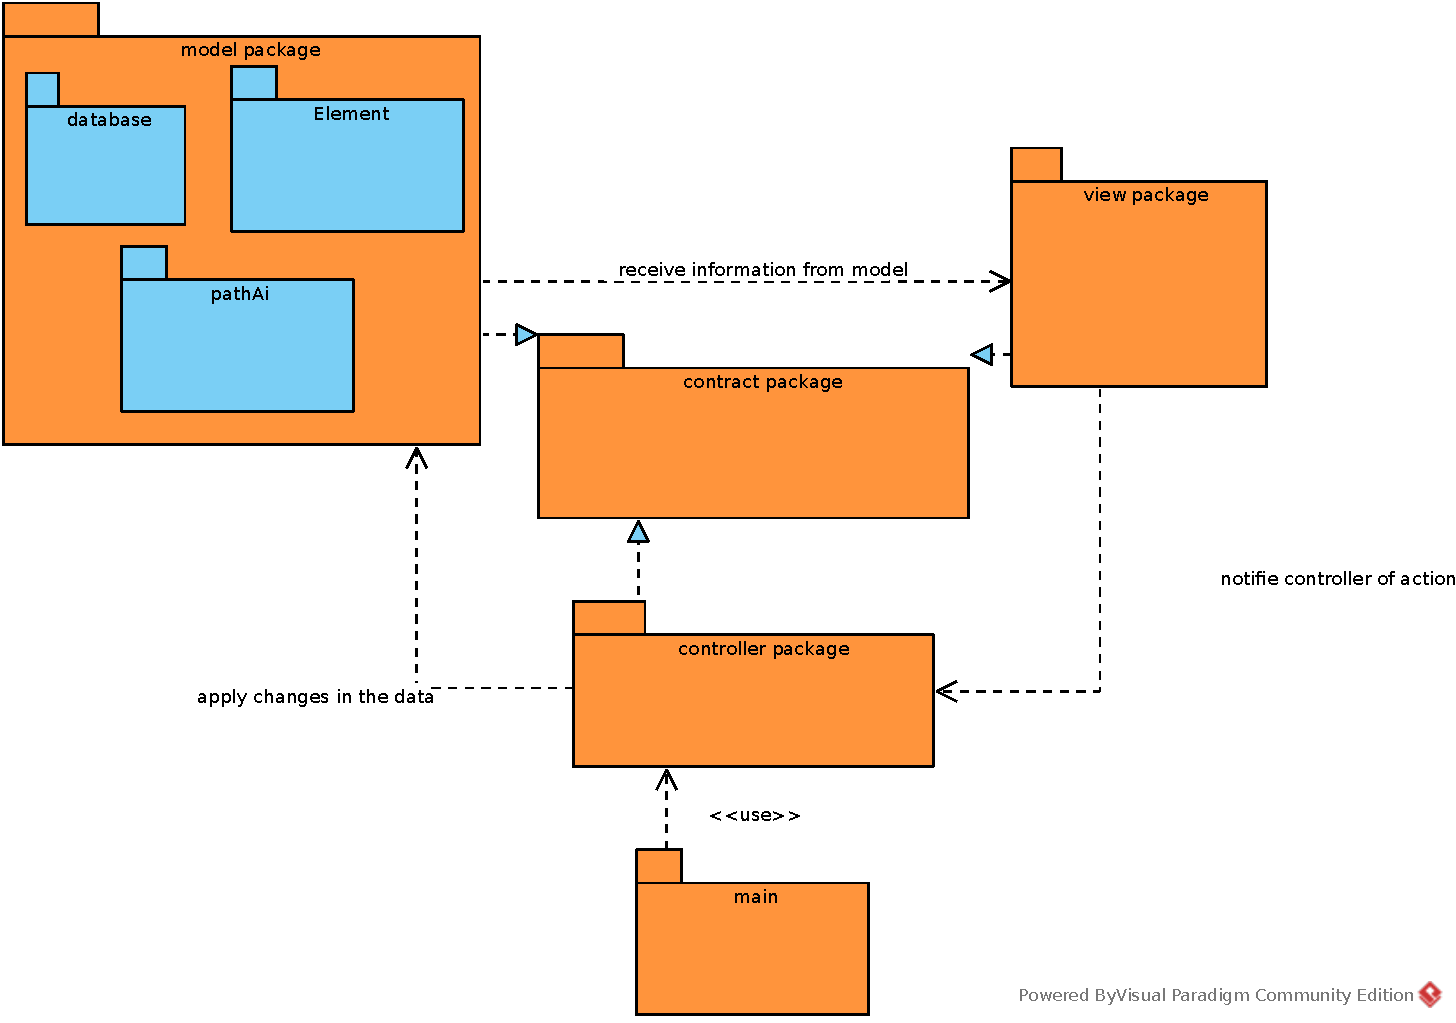
\includegraphics[scale=0.8]{resources/SVG/package.pdf}
\end{center}

\clearpage

\section{Components}

Finally the program’s components are connecting this way

\begin{center}
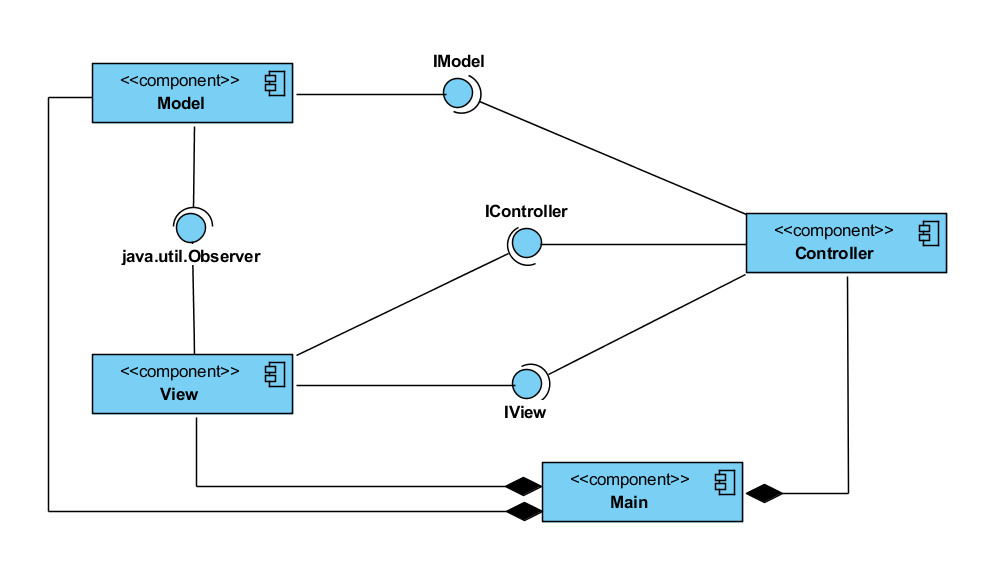
\includegraphics[scale=0.7]{resources/components.png}
\end{center}

\section{Sequence in game}

The program is obeing to the following diagram.

\begin{center}
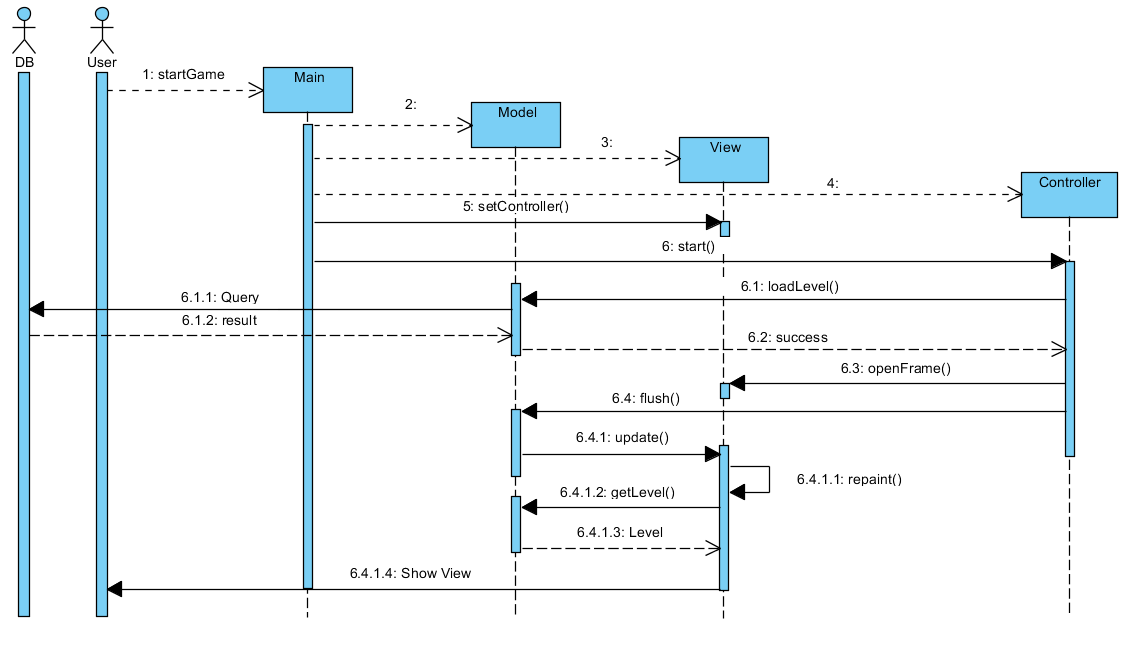
\includegraphics[scale=0.6]{resources/sequence.png}
\end{center}

First the user starts the game, the main will activate the model, the view then the controller. The controller will ask the model to load the first level, the level is charged from the data base and return to the model. Next the controller will make the view open a frame that will the interface with the user. At every player’s action the view will update by charging the model’s data.

\section{Database}

\subsection{Map}

To create the maps first we made a text file were each letter was corresponding to an element of the game. Then with a filling script we fill the database with all the elements and their location (x,y) on the different levels of the game.

\begin{center}
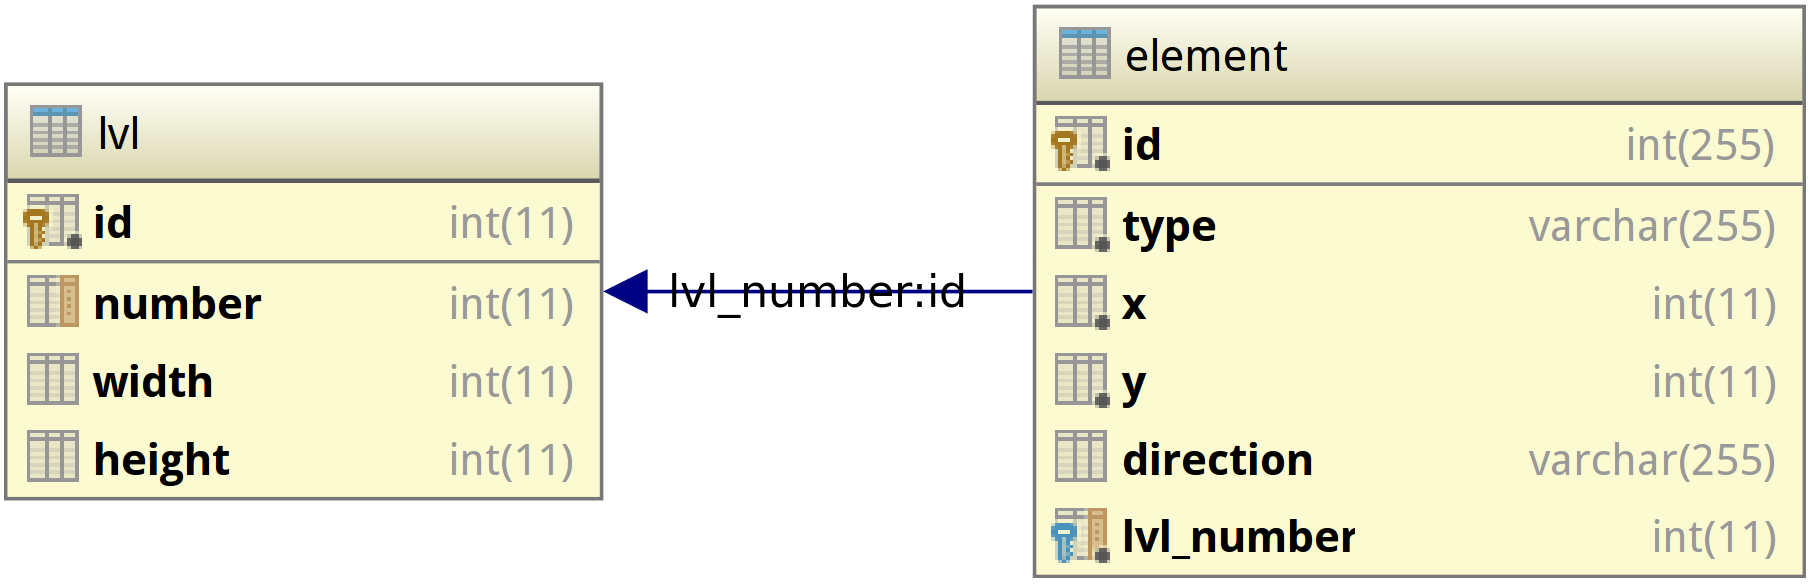
\includegraphics[scale=0.2]{resources/MPD.png}
\end{center}

\section{Stored procedures}

The database is composed of 3 stored procedure to create de different levels.

\paragraph{get\_elements\_by\_level} return all the elements from a specific level

\begin{lstlisting}[language=SQL]
DELIMITER |
CREATE PROCEDURE get_elements_by_level (IN lvlID int)
	BEGIN
		SELECT element.id, element.type, element.x, element.y, element.direction, element.lvl_number FROM element WHERE lvl_number = lvlID
	END |
DELIMITER ;
\end{lstlisting}

\paragraph{get\_levels} return all the levels

\begin{lstlisting}[language=SQL]
DELIMITER |                                                      
CREATE PROCEDURE get_levels
	BEGIN
		SELECT *
		FROM lvl
		ORDER BY lvl.number
	END |
DELIMITER ;
\end{lstlisting}

\paragraph{get\_level\_by\_id} return a specific level

\begin{lstlisting}[language=SQL]
DELIMITER |                                                      
CREATE PROCEDURE get_level_by_id (IN id int)
	BEGIN
		SELECT * FROM lvl WHERE lvl.id = id LIMIT 1
	END |
DELIMITER ;
\end{lstlisting}

\chapter{Reports}

\section{Git}

During this project we made over \emph{180} commits on our repository on GitHub at \texttt{\href{https://github.com/EpicKiwi/Lorann-Ex/}{goo.gl/EyqrgK}}

\subsection{Contributors participation}

This is the contribution of every member of the team based on the number of commits they made.

\begin{multicols}{4}
\begin{description}
\item [Clément] 28,5\ \%
\item [Marie] 15\ \%
\item [Baptiste] 68,8\ \%
\item [Maxime] 3,7\ \%
\end{description}
\end{multicols}

\chapter{Personnal assessment}

\section{Clément Chabrier}

This JAVA project was very interesting yet complicated, I thought that my lacks in this language would be penalizing for the group.

However, with our teamwork we managed to compensate for everyone’s weaknesses and reach our goals.

Through my mission of building the view part I improved my skills on several point about the JAVA language, specifically on software architecture and visual shows on JAVA console.

Also I developed a real complicity with my colleague, Baptiste Saclier, which led us to an optimal development of the project.

\section{Maxime Zupka}

This project was very interesting because it was a very comprehensive one. We had to use Java which is a new language but also other things that we learn during the year such as database. And I really like the idea of remaking an oldschool game. I think we did a great a job and the project is a success. 

\section{Baptiste Saclier}

This project was an opportunity to me to discover the happy things of the team managment and the Java project build. I think all my team was involded in the creation of this game and they wants all to participate.

To conclude, it was a great project with many challenges.

\end{document}